\begin{figure*}[t!]
\centering
\vspace*{-3ex}
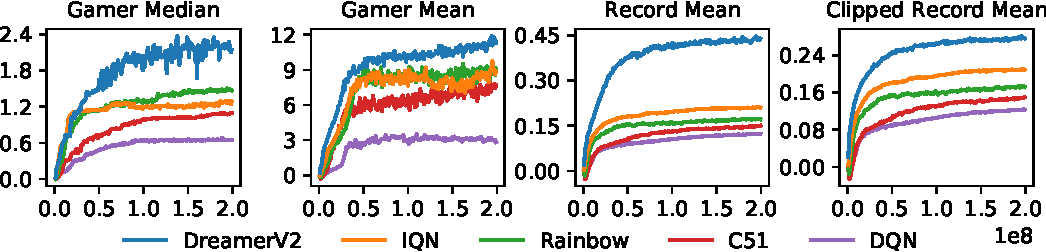
\includegraphics[width=\textwidth]{agg/agg}
\caption{Atari performance over 200M steps. See \cref{tab:agg} for numeric scores. The standards in the literature to aggregate over tasks are shown in the left two plots. These normalize scores by a professional gamer and compute the median or mean over tasks \citep{mnih2015dqn,mnih2016a3c}. In \cref{sec:experiments}, we point out limitations of this methodology. As a robust measure of performance, we recommend the metric in the right-most plot. We normalize scores by the human world record \citep{toromanoff2019atarirecords} and then clip them, such that exceeding the record does not further increase the score, before averaging over tasks.}
\label{fig:agg}
\vspace*{2ex}
\end{figure*}
